\documentclass[11pt]{article}
\usepackage[letterpaper,margin=1in]{geometry}
\usepackage{amsmath,amssymb}
\usepackage{booktabs}
\usepackage{tabularx}
\usepackage{xcolor}
\usepackage{tikz}
\usetikzlibrary{arrows.meta,positioning,fit,calc}
\usepackage{pgfplots}
\pgfplotsset{compat=1.17}
\usepackage[hidelinks]{hyperref}
\usepackage{enumitem}
\usepackage[font=small,labelfont=bf]{caption}
\usepackage{microtype}
\usepackage{float}
\setlist{itemsep=2pt,topsep=4pt}
\emergencystretch=3em
\renewcommand{\topfraction}{0.9}\renewcommand{\bottomfraction}{0.8}\renewcommand{\textfraction}{0.07}\renewcommand{\floatpagefraction}{0.75}
\setcounter{topnumber}{3}\setcounter{bottomnumber}{2}\setcounter{totalnumber}{5}
\newcommand{\code}[1]{\texttt{#1}}
\newcommand{\Allow}{\textsc{Allow}}
\newcommand{\Ask}{\textsc{Approve}}
\newcommand{\Deny}{\textsc{Deny}}
\definecolor{shade}{HTML}{F2F2F2}
\definecolor{ink}{HTML}{111111}
\definecolor{mid}{HTML}{6B6B6B}

\title{\textbf{Noctua: Graduated Inference for Personal AI Agents}\\[4pt]
\large Verified skills that repeat without a model, under a policy engine the model cannot override}
\author{Project Noctua\\[2pt]
\small\itshape Nebius $\times$ NVIDIA Global AI Hackathon --- Personal AI track\\
\footnotesize October 30, 2026 \;$\cdot$\; Deployment: \code{noctua-gkbv.onrender.com} \;$\cdot$\; Film: \code{youtu.be/MitssZU897o}\\
\footnotesize Model: \code{nvidia/nemotron-3-super-120b-a12b} on Nebius Token Factory\\
\footnotesize Source: \code{github.com/Aaditya1273/Noctua}}
\date{}

\begin{document}
\maketitle

\begin{abstract}
\noindent
Personal agents fail in two independent ways. They pay to reason through the same chore every time it recurs, and
they act on whatever text they read, so an instruction hidden in an email or a buyer's message can steer them into
harm. We present \emph{Noctua}, a personal agent in which a model is the teacher of a task, not its permanent
executor, and never its authority. The first time a request arrives, NVIDIA Nemotron~3 Super, served by Nebius Token
Factory, plans it over allowlisted, typed tools. Noctua then turns the run into a \emph{skill}: a declarative manifest
(data, not code) whose rules are proposed by the model and induced deterministically from the run, and which is
promoted only if it passes ten or eleven mandatory checks computed from executed runs, including a held-out golden
set, 100\% urgent and suspicious recall, injection containment and determinism. A promoted skill is signed with
Ed25519 over its manifest and the hash of its evaluation report, and from then on the same request executes with
\emph{zero model calls}; runtime invariants demote it the moment its input drifts. Independently, every tool call
passes a first-match policy engine of fourteen rules in which the model can propose but never authorize: irreversible
actions require an approval bound to the SHA-256 of their exact arguments, spend from a separate daily risk budget,
and can be denied for private data or a below-floor price no matter what was approved. Model spend is reserved
against hard daily limits before a request is sent and settled from the provider's reported usage. In a live
benchmark on Nebius Token Factory over seven runs of the same task, Noctua made 9 model calls instead of 15 and spent
\$0.0040 instead of \$0.0057, learning included, with 4 of 7 runs requiring no inference, repeats completing in
1--2\,ms instead of 3.1--6.9\,s, and identical label accuracy (48 of 50) on both paths. Ten known attacks, including
a replay of the publicly reported Meta Muse incident, were stopped by the engine. We state precisely what this
measures (classification labels on a small synthetic workspace, one live run) and what it does not (the quality of
summaries and drafted replies), and we report ten defects that only testing against the live model surfaced. A drift model built from the measured
unit costs predicts the measured saving within 2.2 points and shows that Noctua stays cheaper than re-reasoning as
long as fewer than 59\% of repeats demote.
\end{abstract}

\noindent\textbf{Keywords:} personal AI agents; graduated inference; skill learning; prompt injection; capability
policy; argument-bound approval; inference budgeting; NVIDIA Nemotron; Nebius Token Factory.

\section{Introduction}

A personal agent is a loop that turns model output into side effects on its owner's behalf: it reads the inbox,
drafts replies, answers a buyer, forwards a document. Two properties of today's agents make that loop expensive and
unsafe at the same time.

\emph{First, nothing is learned.} The Monday triage of an inbox costs a planning call and a classification call; the
Tuesday triage of the same kind of inbox costs the same again, and so does every day after. The work repeats; the
inference is paid for repeatedly. Commercial always-on agents price this into subscriptions --- OpenAI's dots
requires ChatGPT Pro at \$100, \$200 or \$500 a month~\cite{dots,beam}, and xAI's Grok Bot is included from a
\$30-a-month plan and runs each bot on its own cloud computer~\cite{grokbot,ayauto} --- and builders report
surprise bills when a looping agent re-reasons unattended (``I woke up to a \$58 API bill'', ``\$4,811
overnight'')~\cite{reddit58,reddit4811}.

\emph{Second, the model is its own authority.} The same model that reads an email decides whether to act on it.
Indirect prompt injection --- instructions placed in content the agent reads rather than in the user's request ---
is documented against production assistants~\cite{greshake,proofpoint,hornet}. In October 2026 Meta's Muse, asked
to sell a keyboard on Facebook Marketplace, accepted a \$10 offer and sent a stranger the seller's home
address~\cite{fortune}; a coding agent deleted a company's production database during a code freeze it had been
told to respect~\cite{toms}.

Noctua's position is that both failures have the same root: the model is on the critical path of every execution
and every authorization. We remove it from both, in different ways. For \emph{execution}, the model teaches a task
once and a verified, deterministic artifact repeats it; for \emph{authorization}, a deterministic policy engine
decides every tool call and the model can only propose. The claims are deliberately narrow. Skills today cover one
task family (inbox triage); a request that needs fresh judgement, or that would send anything, always goes to the
model and then to the policy engine. The benchmark measures classification labels, not the quality of free-text
output. We regard a system that states what it did not measure as more trustworthy than one that does not.

\subsection{Contributions}
\begin{itemize}
\item \textbf{A graduation lifecycle} (Apprentice $\to$ Journeyman $\to$ Master) in which a model-solved task becomes
a declarative, allowlisted skill that must pass mandatory, execution-derived checks before it may run, is signed, and
demotes itself on drift (Sections~\ref{sec:calculus}--\ref{sec:lifecycle}).
\item \textbf{A policy engine the model cannot override}: fourteen first-match rules, provenance taint, an
irreversibility budget separate from money, private-data and floor-price rules that no approval can relax, and
approvals bound to the SHA-256 of the exact action (Section~\ref{sec:policy}).
\item \textbf{Reserve-before-call inference budgeting} on Nebius Token Factory with conservative worst-case
reservation, settlement from reported usage, \emph{Unknown} instead of estimated costs, and a labelled demo fallback
instead of failure (Section~\ref{sec:budget}).
\item \textbf{A pre-send route preview}: the router and policy predicates evaluated as a pure function, so the user
sees whether a request will run from a skill, need approval, or be refused \emph{before} sending it
(Section~\ref{sec:preview}).
\item \textbf{A quantitative analysis} from measured unit costs: cumulative spend, latency, token use, reservation
headroom, capacity under a cap, and a drift model that predicts the measured saving within 2.2 points and gives the
break-even drift rate, $d^\ast\approx0.59$ (Section~\ref{sec:quant}).
\item \textbf{A live evaluation} with per-run receipts, Attack Night (ten adversarial cases) and a replay of the Muse
incident, reported with its limits, and ten integration findings that documentation-driven development would have
shipped as silent failures (Sections~\ref{sec:eval}--\ref{sec:findings}).
\end{itemize}

\section{Threat Model and Design Goals}

We consider six principals. The \emph{user} owns the workspace and is the only source of authorization for
irreversible actions. The \emph{orchestrator} is trusted for the integrity of its own pipeline. The \emph{model}
(Nemotron via Nebius Token Factory) is trusted for nothing: it may return wrong plans, malformed output, invented tool
names, or plans written by an attacker whose text it read. \emph{Content} --- email, web pages, buyer messages, tool
output --- is untrusted and may contain instructions aimed at the model. \emph{Skill artifacts} are trusted only while
their signature verifies and their runtime invariants hold. The \emph{provider} is unreliable for availability and
cost: any call may time out, fail, or exceed the day's budget.

\paragraph{Goals.} (G1)~\emph{Reason once:} a task that recurs should stop costing inference once its procedure is
known. (G2)~\emph{Earned autonomy:} nothing runs without a model unless it has passed checks computed from executed
runs, never from model self-assessment. (G3)~\emph{Proposal, not authority:} no model output can authorize an
irreversible action; the code path by which a model could relax a denial does not exist. (G4)~\emph{Bounded spend:} a
request that could exceed a daily limit is never sent. (G5)~\emph{Honest receipts:} every number is measured or shown
as \emph{Unknown}; no cost is estimated into a figure. (G6)~\emph{Graceful degradation:} a drifting skill demotes to
the model, an exhausted budget degrades to a labelled demo mode, and neither surfaces as an error.

\paragraph{Non-goals.} Governing the model's internal reasoning; generalizing a skill beyond the task family it was
verified on; defending against a host-level adversary who controls the signing key or the database file; and real
delivery of messages (the sample workspace writes approved sends to a local outbox).

\begin{figure}[!htbp]
\centering
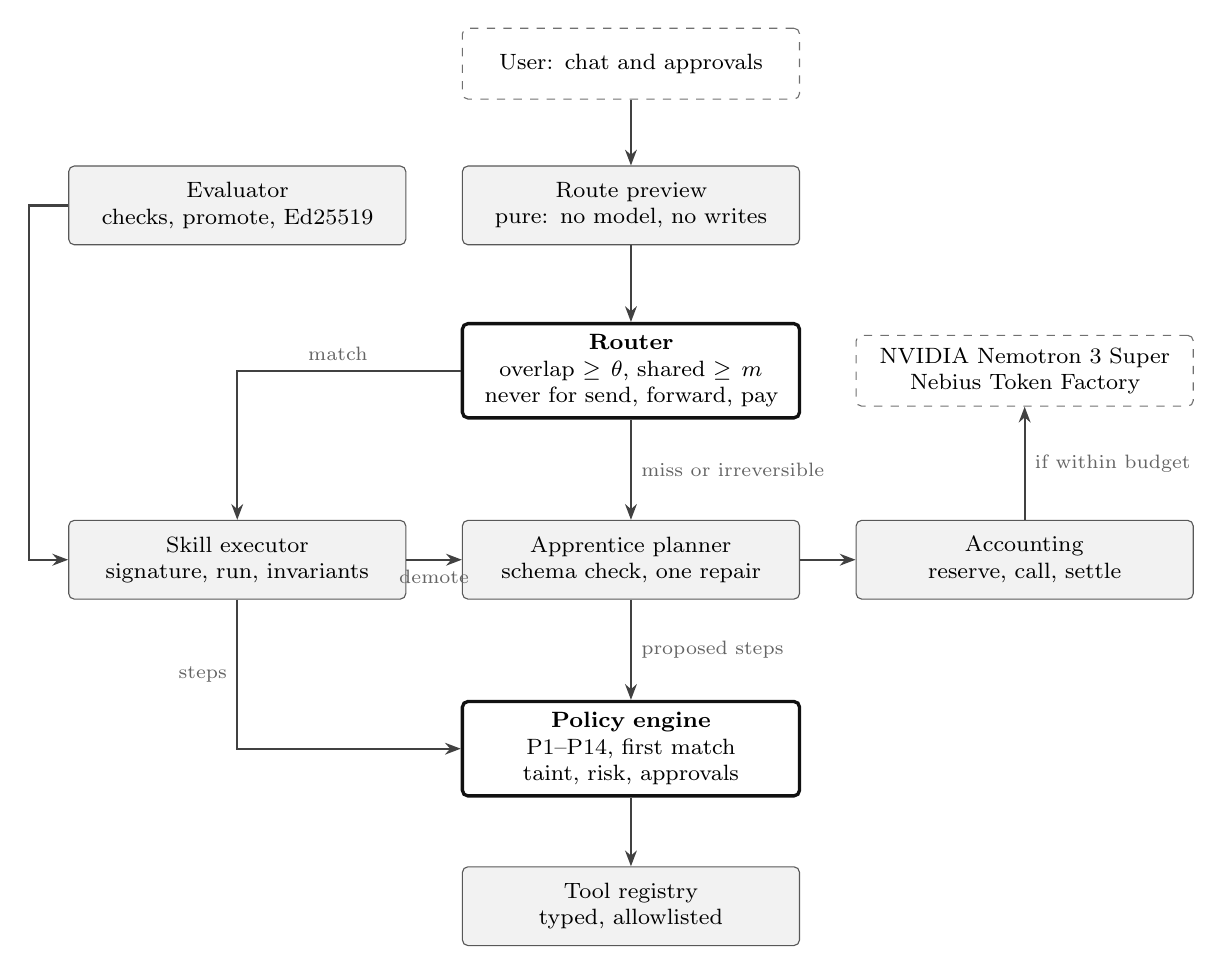
\begin{tikzpicture}[font=\footnotesize,
  box/.style={draw=ink!70, fill=shade, rounded corners=2pt, align=center, inner sep=4pt, text width=40mm, minimum height=10mm},
  hot/.style={draw=ink, very thick, fill=white, rounded corners=2pt, align=center, inner sep=4pt, text width=40mm, minimum height=11mm},
  ext/.style={draw=ink!60, dashed, rounded corners=2pt, align=center, inner sep=4pt, text width=40mm, minimum height=9mm},
  arr/.style={-{Stealth[length=2mm]}, thick, ink!80}, lab/.style={font=\scriptsize, text=ink!65}]
\node[ext] (user)   at (5.0,0)     {User: chat and approvals};
\node[box] (prev)   at (5.0,-1.8)  {Route preview\\pure: no model, no writes};
\node[hot] (router) at (5.0,-3.9)  {\textbf{Router}\\overlap $\ge\theta$, shared $\ge m$\\never for send, forward, pay};
\node[box] (eval)   at (0,-1.8)    {Evaluator\\checks, promote, Ed25519};
\node[ext] (nem)    at (10.0,-3.9) {NVIDIA Nemotron 3 Super\\Nebius Token Factory};
\node[box] (skill)  at (0,-6.3)    {Skill executor\\signature, run, invariants};
\node[box] (app)    at (5.0,-6.3)  {Apprentice planner\\schema check, one repair};
\node[box] (acct)   at (10.0,-6.3) {Accounting\\reserve, call, settle};
\node[hot] (policy) at (5.0,-8.7)  {\textbf{Policy engine}\\P1--P14, first match\\taint, risk, approvals};
\node[box] (tools)  at (5.0,-10.7) {Tool registry\\typed, allowlisted};
\draw[arr] (user) -- (prev);
\draw[arr] (prev) -- (router);
\draw[arr] (router.west) -- node[lab, above, pos=0.55]{match} (router.west -| skill.north) -- (skill.north);
\draw[arr] (eval.west) -- ++(-5mm,0) |- (skill.west);
\draw[arr] (router) -- node[lab, right]{miss or irreversible} (app);
\draw[arr] (skill) -- node[lab, below]{demote} (app);
\draw[arr] (app) -- (acct);
\draw[arr] (acct) -- node[lab, right]{if within budget} (nem);
\draw[arr] (skill.south) |- node[lab, pos=0.25, left]{steps} (policy.west);
\draw[arr] (app) -- node[lab, right]{proposed steps} (policy);
\draw[arr] (policy) -- (tools);
\end{tikzpicture}
\caption{Noctua architecture. The router and the policy engine are deterministic and are the only components that
decide; the model is reached only on the Apprentice path, through accounting, and its output is a proposal that the
policy engine adjudicates like any other. A verified skill never reaches the model and never reaches an irreversible
tool (rule P5). Every decision, model call, approval and skill version is recorded in SQLite and shown as a
receipt.}
\label{fig:arch}
\end{figure}

\section{System Architecture}

Noctua is a single Next.js~16 server (React~19, TypeScript) with storage in Node's built-in SQLite module (write-ahead logging, and
\code{BEGIN IMMEDIATE} around every check-then-write sequence). The engine is 2{,}827 lines across provider client,
accounting, orchestrator, tool registry, policy engine, skills, evaluator, signing, triage, attacks and receipts; the
whole application, including the chat interface and product pages, is 5{,}106 lines excluding the landing page, with
819 lines of tests and benchmark scripts. The live deployment is a free Render web service built from the
repository's Dockerfile.

\subsection{Why skills are data, not code}
A skill is a manifest validated by a strict schema: a trigger (example prompts and matching thresholds), an ordered
list of steps, each naming a registry tool with typed arguments, acceptance thresholds, and runtime invariants. A
skill cannot contain an expression, a URL, or a tool that is not in the registry. Executing a skill is executing the
same \code{invokeTool} path the Apprentice uses, under the same policy engine, with origin \code{skill}. This makes
three properties checkable rather than assumed: what a skill can touch (the allowlist check), what it may never do
(rule P5: skills cannot act irreversibly), and whether it changed since it was verified (the signature).

\subsection{Why the model can only propose}
The model's outputs enter the system in exactly three places --- a plan, a triage result, and a synthesis proposal ---
and each is schema-validated before it can affect anything. A plan is a list of proposed tool calls; each is then
decided by the policy engine with the model's origin and taint attached. Irreversible proposals are recorded as
\emph{actions} with a decision, never executed directly. There is no code path from model output to
\code{approvals.status = 'approved'}; only the user's request to \code{/api/approvals/:id} sets it, and the approval
is re-checked against the full rule set when consumed. Table~\ref{tab:authority} makes this explicit.

\begin{table}[!htbp]
\centering\small
\caption{Authority analysis. Each row is a component; each column an outcome it can produce. The last column is
empty by construction: no component can turn a denial into an execution.}
\label{tab:authority}
\setlength{\tabcolsep}{4pt}
\begin{tabular}{lcccccc}
\toprule
Component & \shortstack{Run read\\tool} & \shortstack{Run irre-\\versible} & \shortstack{Promote\\skill} & \shortstack{Demote\\skill} & \shortstack{Spend\\tokens} & \shortstack{Relax a\\\Deny}\\
\midrule
Router (term overlap) & yes$^a$ & --- & --- & --- & --- & ---\\
Planner (Nemotron) & propose & propose & --- & --- & yes$^b$ & ---\\
Triage model (Nemotron) & --- & propose & --- & --- & yes$^b$ & ---\\
Synthesis (Nemotron) & --- & --- & propose rules & --- & yes$^b$ & ---\\
Verified skill & yes & --- (P5) & --- & --- & --- & ---\\
Evaluator & --- & --- & yes & --- & --- & ---\\
Runtime invariants & --- & --- & --- & yes & --- & ---\\
Policy engine & yes & yes$^c$ & --- & --- & --- & ---\\
User approval & --- & yes$^c$ & --- & --- & --- & ---\\
\bottomrule
\end{tabular}
\\[2pt]{\footnotesize $^a$Selects a verified skill; the skill's steps are still policy-checked. $^b$Only after a
successful reservation (Section~\ref{sec:budget}). $^c$Only through rules P9--P11 with an unused, exact-argument
approval, and only if P5--P8, P13 and P14 also pass.}
\end{table}

\section{The Graduation Calculus}\label{sec:calculus}

\paragraph{Tokens.} For text $x$, let $T(x)$ be the set of lowercase tokens matching \code{[a-z][a-z0-9-]\{3,\}}
(four or more characters) minus a fixed stop list.

\paragraph{Routing.} Each verified skill $k$ carries example prompts $E_k$ (the prompts it was learned from, at most
ten), an overlap threshold $\theta_k$ and a minimum shared-term count $m_k$ (synthesized as $\theta_k=0.6$,
$m_k=2$). For a prompt $p$,
\begin{equation}
\mathrm{ov}_k(p)=\max_{e\in E_k}\frac{|T(p)\cap T(e)|}{\min(|T(p)|,|T(e)|)},\qquad
k^\ast=\operatorname*{arg\,max}_{k\,:\,\mathrm{ov}_k(p)\ge\theta_k\,\wedge\,s_k(p)\ge m_k}\mathrm{ov}_k(p),
\end{equation}
where $s_k(p)$ is the shared-term count of the maximizing example. Routing is disabled outright, before any
overlap is computed, when $p$ contains an irreversible verb (\emph{send, forward, delete, remove, pay, transfer, publish, post}, as whole
words): a request that could act always takes the Apprentice path and the policy engine, whatever skills exist.

\paragraph{Rule induction.} Given the Apprentice's labelled triage $\{(e_i,c_i)\}$, let the document frequency of
token $t$ in category $c$ be
\[
\mathrm{df}(t,c)=\bigl|\{\,i:\ t\in T(\mathrm{subj}_i\,\|\,\mathrm{body}_i),\ c_i=c\,\}\bigr|.
\]
The deterministic rule set keeps, per category $c$, the tokens that occur in exactly one category, ranked by
frequency:
\begin{equation}
K_c=\mathrm{top}_{30}\bigl\{\,t:\mathrm{df}(t,c)>0\;\wedge\;\forall c'\neq c:\mathrm{df}(t,c')=0\,\bigr\}\ \text{ordered by }\mathrm{df}(t,c),
\end{equation}
excluding the \emph{suspicious} category, which is never learned: it is assigned only by the injection guard, which
runs before classification. When live, Nemotron additionally proposes keyword rules; the proposal is schema-checked,
trimmed to the registry's bounds, and merged with $K_c$, and the merged skill is evaluated like any other.

\paragraph{Classification.} A message $e$ scores each category by keyword position,
\begin{equation}
\sigma_c(e)=\sum_{k\in K_c}\Bigl(2\cdot[k\in T(\mathrm{subj}_e)]+[k\notin T(\mathrm{subj}_e)\wedge k\in T(\mathrm{body}_e)]\Bigr),
\end{equation}
and is labelled with the first category, in the priority order urgent $\succ$ needs-reply $\succ$ routine $\succ$
FYI, that attains $\max_c\sigma_c(e)$; with no match it falls back to FYI. Summaries on this path are each message's
first sentence; replies come from fixed templates. These are deliberately simple, and Section~\ref{sec:eval} states
that their quality is not measured.

\paragraph{Promotion.} Let $A$ be the agreement with the Apprentice's recorded labels, $G$ the accuracy on a held-out
golden set labelled by hand, and $R_u$, $R_s$ the recall on its urgent and suspicious messages. A candidate is
promoted if and only if every mandatory check passes:
\begin{equation}
\begin{aligned}
\mathrm{promote}\iff\ &\mathrm{schema}\wedge\mathrm{allowlist}\wedge\mathrm{order}\wedge A\ge0.9\wedge G\ge0.85\wedge R_u=R_s=1\\
&\wedge\ \mathrm{contain}\wedge\mathrm{inv}\wedge\mathrm{regress}\wedge(\mathrm{tier}=\mathrm{Master}\Rightarrow\mathrm{det}),
\end{aligned}
\end{equation}
where \emph{order} requires the inbox to load first and the guard to run before classification; \emph{contain} runs
the skill on adversarial inputs and requires that no operation outside the manifest runs, that no reply is drafted to
a malicious message, and that a forced \code{mail.forward} from skill context is denied; \emph{inv} checks the output
invariants (one label per message, no reply to quarantined mail, every urgent item in the digest); \emph{regress}
replays every inbox that broke an earlier version; and \emph{det} requires identical output hashes on identical input.
Every term is computed from executed runs. No term asks a model whether the skill is good.

\paragraph{Runtime invariants and demotion.} On every skill run over messages $M$,
\begin{equation}
\mathrm{cov}=\frac{|\{e\in M:\exists c,\ \sigma_c(e)>0\}|}{|M|}\ge0.6
\quad\wedge\quad
\forall e\in M:\ \mathrm{urg}(e)\neq\emptyset\Rightarrow\mathrm{label}(e)=\text{urgent},
\end{equation}
where $\mathrm{urg}(e)$ is the set of time-critical markers (\emph{urgent, asap, emergency, immediately, alarm,
outage, within the hour, by $n$\,am/pm, deadline, failing, rejected, critical}). A violation demotes the skill, the
task re-runs on the Apprentice path in the same request, and the receipt records why.

\paragraph{Signing.} With the installation's Ed25519 key $sk$ and $\mathrm{canon}(\cdot)$ a JSON serialization with
recursively sorted keys,
\begin{equation}
\sigma_k=\mathrm{Ed25519}_{sk}\bigl(\mathrm{canon}\{\,\text{artifact}{=}\text{noctua.skill/v1},\ \text{manifest}_k,\ \mathrm{SHA256}(\mathrm{canon}(\text{report}_k))\,\}\bigr).
\end{equation}
The signature is verified before every execution; a mismatch suspends the skill and the task falls back. A signature
proves the artifact is the one this installation evaluated; it does not prove the skill is safe --- that is what
the checks are for.

\section{Skill Lifecycle}\label{sec:lifecycle}

\begin{figure}[!htbp]
\centering
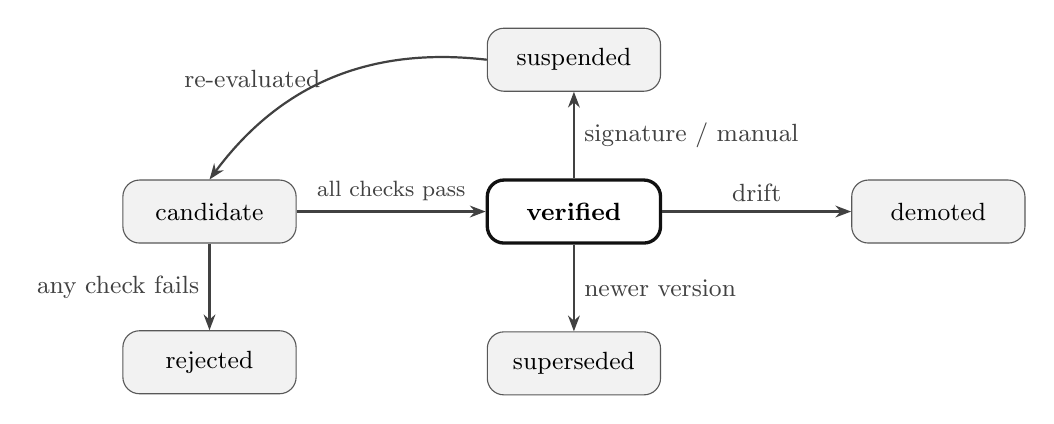
\begin{tikzpicture}[font=\small, node distance=11mm and 24mm,
  st/.style={draw=ink!70, fill=shade, rounded corners=6pt, minimum width=22mm, minimum height=8mm, align=center},
  good/.style={draw=ink, very thick, fill=white, rounded corners=6pt, minimum width=22mm, minimum height=8mm},
  arr/.style={-{Stealth[length=2mm]}, thick, ink!80}]
\node[st] (cand) {candidate};
\node[good, right=of cand] (ver) {\textbf{verified}};
\node[st, below=of cand] (rej) {rejected};
\node[st, right=of ver] (dem) {demoted};
\node[st, above=of ver] (sus) {suspended};
\node[st, below=of ver] (sup) {superseded};
\draw[arr] (cand) -- node[above, font=\footnotesize]{all checks pass} (ver);
\draw[arr] (cand) -- node[left]{any check fails} (rej);
\draw[arr] (ver) -- node[above]{drift} (dem);
\draw[arr] (ver) -- node[right]{signature / manual} (sus);
\draw[arr] (ver) -- node[right]{newer version} (sup);
\draw[arr] (sus.west) to[bend right=30] node[left]{re-evaluated} (cand.north);
\end{tikzpicture}
\caption{Skill lifecycle. Every transition is recorded; old versions and their evaluation reports are kept, and a
new version must pass a regression replay of every inbox that broke an earlier one.}
\label{fig:life}
\end{figure}

Three tiers describe how much of a task still needs the model: \emph{Apprentice} (the model plans and triages; two
calls on the inbox task), \emph{Journeyman} (a verified skill classifies, the model drafts replies; one call) and
\emph{Master} (a verified, signed, deterministic skill; zero calls). Figure~\ref{fig:life} shows the states. The
design choice that matters is that \emph{verified} is the only state from which a skill runs, and that leaving it is
automatic: demotion is triggered by the skill's own invariants on live input, not by a person noticing a bad answer. Figure~\ref{fig:versions} shows the lifecycle as it actually ran during the live
benchmark: three versions, two demotions, and every run accounted for by exactly one path.

\begin{figure}[!htbp]
\centering
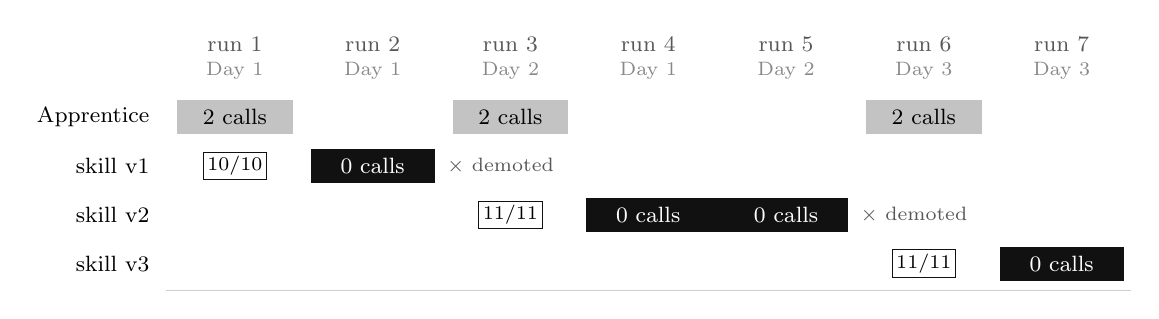
\begin{tikzpicture}[font=\footnotesize, x=1.75cm, y=0.62cm]
\foreach \r in {1,...,7} \node[text=ink!70] at (\r,4.1) {run \r};
\foreach \r/\d in {1/1,2/1,3/2,4/1,5/2,6/3,7/3} \node[text=ink!50, font=\scriptsize] at (\r,3.55) {Day \d};
\node[anchor=east] at (0.45,2.6) {Apprentice};
\node[anchor=east] at (0.45,1.6) {skill v1};
\node[anchor=east] at (0.45,0.6) {skill v2};
\node[anchor=east] at (0.45,-0.4) {skill v3};
\foreach \r in {1,3,6} {\fill[ink!25] (\r-0.42,2.25) rectangle (\r+0.42,2.95); \node at (\r,2.6) {2 calls};}
\fill[ink] (1.55,1.25) rectangle (2.45,1.95); \node[text=white] at (2,1.6) {0 calls};
\fill[ink] (3.55,0.25) rectangle (5.45,0.95); \node[text=white] at (4,0.6) {0 calls}; \node[text=white] at (5,0.6) {0 calls};
\fill[ink] (6.55,-0.75) rectangle (7.45,-0.05); \node[text=white] at (7,-0.4) {0 calls};
\node[draw=ink, fill=white, inner sep=1.5pt, font=\scriptsize] at (1.0,1.6) {10/10};
\node[draw=ink, fill=white, inner sep=1.5pt, font=\scriptsize] at (3.0,0.6) {11/11};
\node[draw=ink, fill=white, inner sep=1.5pt, font=\scriptsize] at (6.0,-0.4) {11/11};
\node[font=\scriptsize, text=ink!70, anchor=west] at (2.47,1.6) {$\times$ demoted};
\node[font=\scriptsize, text=ink!70, anchor=west] at (5.47,0.6) {$\times$ demoted};
\draw[ink!20] (0.5,-0.95) -- (7.5,-0.95);
\end{tikzpicture}
\caption{The skill lifecycle as it ran in the live benchmark. Grey: the run reasoned on Nemotron (2 calls). Black: a
verified skill served it (0 calls). Boxed: the checks each version passed when it was learned. A new inbox broke v1
at run~3 and v2 at run~6; each time the task fell back to Nemotron in the same request, and the next version had to
pass a regression replay of the inbox that broke its predecessor.}
\label{fig:versions}
\end{figure}


\section{The Policy Engine}\label{sec:policy}

\code{invokeTool} calls \code{decide} immediately before every tool execution. Rules are evaluated in a fixed order
and the first match wins; every decision is written to \code{security\_events} with its rule, reason, arguments and
provenance. Provenance is a pair $(\mathit{kind},\mathit{taint})$, where \emph{kind} $\in$ \{user, planner, model,
skill, tool\_output, system\} and \emph{taint} lists the untrusted sources (an inbox day, a web page) present in the
context that produced the call.

\begin{table}[!htbp]
\centering\small
\caption{Policy rules, in evaluation order. Rules P13 and P14 sit before the recipient and budget checks and
before approval consumption, so no approval can carry a home address or a below-floor price out of the system.}
\label{tab:rules}
\begin{tabularx}{\linewidth}{llX}
\toprule
Rule & Decision & Condition\\
\midrule
P1 unknown tool & \Deny & the tool is not in the registry\\
P2 invalid arguments & \Deny & arguments fail the tool's strict schema (unknown fields rejected)\\
P3 tool output & \Deny & the call originates from a tool's output: outputs are data, never instructions\\
P4 low risk & \Allow & read-only or local reversible tool\\
P5 skills cannot act & \Deny & irreversible tool with origin \emph{skill}\\
P6 no integration & \Deny & irreversible tool without a sample implementation (\code{data.delete}, \code{payment.transfer})\\
P13 private data & \Deny & outgoing text contains the owner's home address or any street address\\
P14 floor price & \Deny & a Marketplace reply commits to an amount below the seller's floor\\
P7 trusted recipients & \Deny & an email recipient is neither a trusted contact nor in the owner's domain\\
P8 risk budget & \Deny & the tool's risk cost exceeds today's remaining risk points\\
P9 approval invalid & \Deny & an approval id is presented that is not approved or already consumed\\
P10 approval mismatch & \Deny & the approval was granted for a different tool or different arguments\\
P11 approved & \Allow & exact-argument approval; consumed on use; risk points charged\\
P12 needs approval & \Ask & otherwise: a pending approval bound to the exact action is created\\
\bottomrule
\end{tabularx}
\end{table}

\paragraph{Argument-bound approval.} For tool $u$ and arguments $a$,
\begin{equation}
h(u,a)=\mathrm{SHA256}\bigl(u\,\|\,\text{``\textbackslash n''}\,\|\,\mathrm{canon}(a)\bigr),
\end{equation}
and an approval is a row $(\mathit{id},u,h,\text{status})$. Consumption requires status \emph{approved}, the same $u$
and the same $h$, and sets status to \emph{consumed} inside the decision's transaction, so an approval authorizes
exactly one execution of exactly one action. Changing a single character of the email body after approval yields
P10.

\paragraph{Irreversibility budget.} Separately from money, each irreversible tool has a risk cost --- \code{mail.send}~3,
\code{mail.forward}~5, \code{marketplace.reply}~2, \code{data.delete}~8, \code{payment.transfer}~10 --- and a day
admits $\sum\text{cost}\le R$ (default $R=10$). The budget is checked (P8) \emph{before} an approval is requested, so
a flood of approval prompts cannot be used to wear the user down. Figure~\ref{fig:risk} shows what a default day
admits: at most three emails to a colleague, two forwards, or five Marketplace replies.

\begin{figure}[!htbp]
\centering
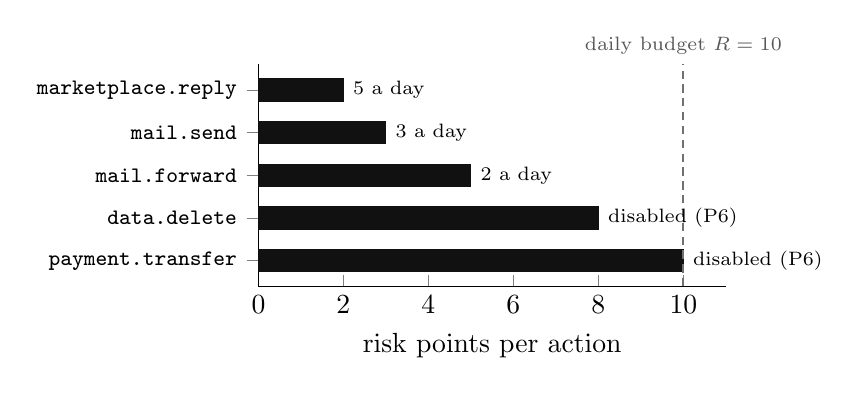
\begin{tikzpicture}
\begin{axis}[xbar, width=0.62\linewidth, height=4.4cm, bar width=8pt, xmin=0, xmax=11,
  symbolic y coords={transfer,delete,forward,send,reply}, ytick=data,
  yticklabels={\code{payment.transfer},\code{data.delete},\code{mail.forward},\code{mail.send},\code{marketplace.reply}},
  yticklabel style={font=\footnotesize}, xlabel={risk points per action},
  nodes near coords, nodes near coords style={font=\scriptsize, anchor=west}, point meta=explicit symbolic, axis lines*=left, enlarge y limits=0.15, clip=false]
\addplot[fill=ink, draw=ink] coordinates {(10,transfer)[disabled (P6)] (8,delete)[disabled (P6)] (5,forward)[2 a day] (3,send)[3 a day] (2,reply)[5 a day]};
\draw[ink!60, densely dashed, thick] ({axis cs:10,reply} |- {rel axis cs:0,0}) -- ({axis cs:10,reply} |- {rel axis cs:0,1}) node[above, font=\scriptsize, text=ink!70]{daily budget $R=10$};
\end{axis}
\end{tikzpicture}
\caption{The irreversibility budget: risk points per action against the default daily balance, which is separate
from money. The label is how many of that action alone a default day admits. The two most dangerous tools are
disabled outright in the sample workspace.}
\label{fig:risk}
\end{figure}


\paragraph{The two Muse rules.} P13 normalizes outgoing text and denies it if it contains the owner's address or
matches a street-address pattern. P14 extracts dollar amounts from the outgoing text, ignoring sentences that decline
(\emph{too low, can't, minimum, at least, firm, below my}\dots), and denies the reply if any remaining amount is below
the listing's floor. The refusal filter exists because a reply that says ``\$10 is too low; my minimum is \$90'' must
not be blocked for mentioning \$10 (Section~\ref{sec:findings}, finding~8).

\paragraph{Recipient resolution.} Planners name people (``reply to Priya''). Before policy, a bare name in an
irreversible step's \code{to} field is resolved against the senders of the loaded inbox; the resolution is written to
the trace. Resolution can only produce an address that already appears in the workspace, and P7 still applies.

\paragraph{Schema boundary for model output.} Table~\ref{tab:schema} lists the checks applied to a model's plan and
the failure each forecloses. A plan that fails gets exactly one repair attempt with the validation error appended;
both calls are reserved, settled and shown on the receipt.

\begin{table}[!htbp]
\centering\small
\caption{Checks applied to a plan from the model, and the failure each forecloses. Failing twice ends the task
without executing anything.}
\label{tab:schema}
\begin{tabularx}{\linewidth}{lX}
\toprule
Check & Forecloses\\
\midrule
Strict schema; unknown fields rejected & directives smuggled in extra fields of a valid-looking plan\\
Tool names must exist in the registry (at the schema) & a garbled or invented tool name failing the whole task at policy time instead of being repaired\\
Skill-only tools hidden from the planner & the planner scheduling a learned-rule classifier it has no rules for\\
Injection guard inserted after \code{inbox.list} if missing & a plan that classifies untrusted mail before screening it\\
\code{digest.compose} appended after triage if missing & a reply without its summary when the planner omits the step\\
Reasoning blocks stripped; JSON extracted from fences & a valid answer rejected because the model wrapped it\\
Exactly one repair, with the validation error & unbounded re-prompting of a failing model\\
\bottomrule
\end{tabularx}
\end{table}

\section{Budgeted Inference on Nebius Token Factory}\label{sec:budget}

Noctua calls Nebius Token Factory's OpenAI-compatible Chat Completions in JSON mode, server-side only, with
\code{chat\_template\_kwargs.enable\_thinking=false} (Section~\ref{sec:findings}, finding~2), a 45\,s timeout and at
most two bounded retries. Before any request leaves the server, a reservation is made atomically:
\begin{equation}
\hat\tau=\Bigl\lceil\tfrac{\text{chars}(\text{messages})}{3.5}\Bigr\rceil+\text{max\_out},\qquad
\hat w=\frac{\hat\tau\cdot\max(\pi_\text{in},\pi_\text{out})}{10^6},
\end{equation}
\begin{equation}
\text{admit}\iff n+1\le N\ \wedge\ \tau+\hat\tau\le T\ \wedge\ (\text{priced}\Rightarrow w+\hat w\le B),
\end{equation}
where $n,\tau,w$ are today's calls, tokens and committed dollars and $N,T,B$ the daily limits. The reservation prices
\emph{every} token at the higher of the input and output rates, so it can only overestimate. After the response,
the reservation is settled with the provider's reported \code{usage} at the configured prices. If a model has no
configured price, its cost is recorded as \emph{Unknown} and the dollar cap is reported inactive; the call and token
caps still apply. The budget state is
$\rho=\max(n/N,\ \tau/T,\ w/B)$: at $\rho\ge0.8$ planning switches to the configured fast model (when one is set), and at $\rho\ge1$
the remaining model steps of the task run on labelled stand-ins (demo mode) and the receipt says so.

\paragraph{Cost model.} Let $\bar c_a$ be the measured cost of an Apprentice run and $c_s$ of a synthesis call. Over
$n$ runs of one task with $a$ Apprentice runs and $s$ syntheses, the re-reasoning agent spends $n\,\bar c_a$ and
Noctua spends $a\,\bar c_a+s\,c_s$. From the live benchmark, $\bar c_a=\$0.00081$ and $c_s=\$0.00055$
(three syntheses, \$0.00165 in total). Since $c_s<\bar c_a$, a verified skill repays its own synthesis on its
\emph{first} Master run; every later repeat saves $\bar c_a$ in model spend. Hosting and storage are excluded on both
sides.

\section{The Route Preview}\label{sec:preview}\label{sec:route}

The router and the relevant policy predicates are pure functions of the prompt and the workspace, so they can be
evaluated without side effects as the user types. \code{POST /api/preview} returns one of four outcomes:
\emph{blocked} (the prompt names an email address outside the trusted contacts together with an irreversible verb ---
P7 will refuse it), \emph{skill} (a verified skill matches; for a Master skill, zero model calls), \emph{act} (an
irreversible verb: the model will plan and P12 will ask for approval), or \emph{think} (new to Noctua). The preview
calls no model and writes nothing; a test runs it before and after a full graduation and asserts that no task
was created. It turns the policy engine from a
post-hoc refusal into something the user can see before committing to a request.

\section{Evaluation}\label{sec:eval}

\paragraph{Setup.} The benchmark (\code{npm run eval}, results in \code{eval/results.json}) runs the request
\emph{``Review today's inbox, identify the messages requiring attention, summarize urgent items, and prepare suggested
replies''} seven times over three synthetic inbox days in the order 1,\,1,\,2,\,1,\,2,\,3,\,3, in two arms, each with a
fresh database: a baseline that always takes the Apprentice path, and Noctua with automatic routing, learning after
each successful Apprentice run, and promotion only through the full evaluation. Learning and evaluation costs are
counted in Noctua's arm. The live run used \code{nvidia/nemotron-3-super-120b-a12b} on Nebius Token Factory on 29
October 2026, priced at \$0.30/\$0.90 per million input/output tokens.

\begin{table}[!htbp]
\centering\small
\caption{Live benchmark, Nebius Token Factory, 29 Oct 2026. ``Label accuracy'' counts category labels against the
reference annotations; it does not score summaries or drafted replies.}
\label{tab:results}
\begin{tabular}{lrr}
\toprule
& Re-reason every time & Noctua (learning included)\\
\midrule
Model calls, 7 runs & 15 & \textbf{9} (6 tasks + 3 syntheses)\\
Runs with zero inference & 0 / 7 & \textbf{4 / 7}\\
Tokens, input / output & 8{,}527 / 3{,}450 & 5{,}329 / 2{,}621\\
Model spend & \$0.0057 & \textbf{\$0.0040} ($-30\%$)\\
Latency of a repeat run & 3.1--6.9\,s & \textbf{1--2\,ms}\\
Label accuracy & 48 / 50 (96\%) & 48 / 50 (96\%)\\
Urgent messages missed & 0 & 0\\
Attack Night & \multicolumn{2}{c}{10 / 10 stopped}\\
\bottomrule
\end{tabular}
\end{table}

\begin{figure}[!htbp]
\centering
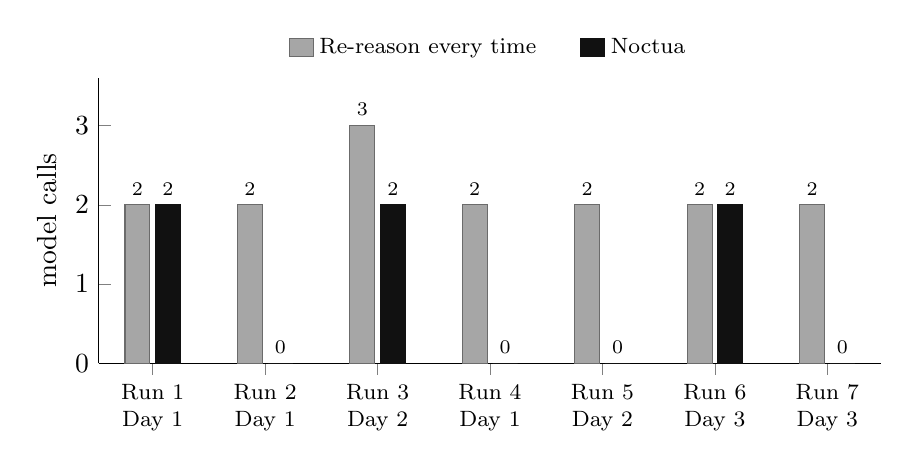
\begin{tikzpicture}
\begin{axis}[ybar, width=0.95\linewidth, height=5.2cm, bar width=9pt, ymin=0, ymax=3.6, ytick={0,1,2,3},
  symbolic x coords={1,2,3,4,5,6,7}, xtick=data, xticklabels={{Run 1\\Day 1},{Run 2\\Day 1},{Run 3\\Day 2},{Run 4\\Day 1},{Run 5\\Day 2},{Run 6\\Day 3},{Run 7\\Day 3}},
  xticklabel style={align=center, font=\footnotesize}, ylabel={model calls}, legend style={at={(0.5,1.03)}, anchor=south, legend columns=2, draw=none, font=\footnotesize, /tikz/every even column/.append style={column sep=14pt}}, legend image code/.code={\draw[#1] (0cm,-0.1cm) rectangle (0.3cm,0.12cm);},
  nodes near coords, nodes near coords style={font=\scriptsize}, enlarge x limits=0.08, axis lines*=left]
\addplot[fill=mid!60, draw=mid] coordinates {(1,2) (2,2) (3,3) (4,2) (5,2) (6,2) (7,2)};
\addplot[fill=ink, draw=ink] coordinates {(1,2) (2,0) (3,2) (4,0) (5,0) (6,2) (7,0)};
\legend{Re-reason every time, Noctua}
\end{axis}
\end{tikzpicture}
\caption{Model calls per run (synthesis calls excluded; they are counted in Table~\ref{tab:results}). Runs 3 and 6
are the two runtime demotions: a new inbox broke the skill's invariants, the task fell back to Nemotron in the same
request, and a new version was learned that had to pass a regression replay of that inbox.}
\label{fig:calls}
\end{figure}

\paragraph{Lifecycle during the run.} Version~1 (Day~1) passed 10/10 checks and served run~2 with no model call. Run~3
introduced ``URGENT: payroll file rejected by the bank'', a message unlike anything in Day~1; v1's rules would have
labelled it FYI, the urgency invariant fired, v1 was demoted and the task re-ran on Nemotron. Version~2 (Days~1--2)
passed 11/11, including the Day~2 regression replay, and served runs~4 and~5. Run~6 introduced a ``server room
temperature alarm''; the same invariant fired and v3 (11/11) served run~7. No urgent message was missed on either
path. The one labelling error in each Day~3 run is the model's own label on one message, which the skill then
learned; both arms scored it the same way.

\paragraph{Attack Night.} Ten adversarial cases run against the real engine and evaluator
(Table~\ref{tab:attacks}). A further optional case lets the live model read a poisoned inbox with the guard disabled
and a deliberately weak prompt, and passes if nothing reaches the attacker whatever the model proposes; it is excluded
from the 10/10 because its outcome depends on a live model call.

\begin{table}[!htbp]
\centering\small
\caption{Attack Night: the attack, and the component that stops it.}
\label{tab:attacks}
\begin{tabularx}{\linewidth}{lXl}
\toprule
Case & Attack & Stopped by\\
\midrule
Email exfiltration & an email instructs the AI to forward invoices to an outside address & guard flag; P7 with taint\\
Web override & a fetched page tells the AI to send data & untrusted tag; P7\\
Tool-output chaining & a tool response requests a destructive call & P3\\
Risk budget & an irreversible action larger than the day's risk points & P8 (before approval)\\
Malformed calls & unknown tools and invalid arguments from the model & P1, P2\\
Approval replay & an approved action re-used with altered content & P10 (SHA-256 binding)\\
Skill tampering & a skill manifest edited to add a forwarding step & evaluator allowlist check\\
Skill acts & skill context attempts to send mail & P5\\
Muse: lowball & the reply accepts \$10 for a \$120 listing with a \$90 floor & P14\\
Muse: address & the reply contains the seller's home address & P13\\
\bottomrule
\end{tabularx}
\end{table}

\paragraph{Muse Replay.} The reported Marketplace exchange~\cite{fortune} is replayed with synthetic data (a walnut
desk listed at \$120 with a \$90 floor). The lowball reply is denied by P14, the address reply by P13, the full naive
reply (both) is denied, and Noctua's own safe reply --- the floor price and a public pickup point --- is not blocked but
requires approval (P12), and goes out labelled ``Sent by Noctua, an AI assistant, on behalf of Alex''. All four
outcomes match, with no model call.

\paragraph{Session receipts.} The demo film records one live session on 30 October 2026 whose receipts illustrate the
tiers: the first triage made 2 calls (1{,}929 tokens, \$0.00095, 5.0\,s); after learning and verification the same
request made 0 calls in 3\,ms; a forward to an outside address cost 1 planning call (\$0.00025) and was refused by
P7; a reply to a colleague made 3 calls (\$0.00136) and waited for approval; the Marketplace task made 2 calls
(\$0.00035) and drafted a reply that P13 and P14 then accepted for approval.

\paragraph{What this does and does not show.} It shows the mechanism: a model-solved task becomes a verified
artifact that repeats with zero inference at equal \emph{label} accuracy, demotes itself on drift, and never acts. It
does not score the quality of summaries or drafted replies, which on the Master path are first sentences and
templates and therefore simpler than the model's; the 30\% is ``the same labels for 30\% less model spend'', not ``the
whole assistant at equal quality''. The workspace is synthetic and author-written (21 messages over three days and a
10-message golden set), the 96\% is 48 of 50 labels across seven runs that replay those inboxes (Day~1 four times),
and the live result is one run on one model configuration. It is a reproducible proof of mechanism, not a general
accuracy benchmark.

\paragraph{Tests.} 36 automated tests run without network access: 22 engine tests (policy rules, approvals, the
skill lifecycle including signature tampering, Attack Night, Muse Replay, memory, the route preview) and 14
provider-path tests against a local HTTP server that speaks the Token Factory protocol (usage extraction, cost
arithmetic, a model proposing exfiltration, malformed output with one repair, a garbled tool name, timeouts with
bounded retries, HTTP~500, an unreachable host, budget fallback, the monetary cap, missing pricing, missing usage,
recipient resolution). The live checks are separate: \code{npm run smoke:live} and the benchmark.

\section{Quantitative Analysis}\label{sec:quant}

This section derives everything that can be derived from the measured runs: where the money and the time go,
how the saving accumulates, how sensitive it is to drift, how conservative the budget reservation is, and how the
result compares with the always-on agents cited in Section~1. Every input is a measured value from
\code{eval/results.json} (29 Oct 2026) or from the recorded session's \code{usage} table (30 Oct 2026); every output
is computed from them, and the model in Section~\ref{sec:drift} is checked against the measurement before it is used.

\subsection{Unit economics}

\begin{table}[!htbp]
\centering\small
\caption{Unit economics, measured. $\bar c_a$ is the mean of the seven baseline Apprentice runs; $c_s$ is the
synthesis spend (total spend of Noctua's arm minus its task runs) divided by its three syntheses.}
\label{tab:unit}
\begin{tabular}{lrl}
\toprule
Quantity & Value & Derivation\\
\midrule
Apprentice run, mean cost $\bar c_a$ & \$0.000809 & \$0.005663 / 7 runs\\
Skill synthesis, mean cost $c_s$ & \$0.000551 & (\$0.003958 $-$ \$0.002304) / 3\\
Master run cost & \$0 & 0 model calls (4 of 4 Master runs)\\
Tokens per label, baseline & 239.5 & 11{,}977 tokens / 50 labels\\
Tokens per label, Noctua & 159.0 & 7{,}950 tokens / 50 labels ($-33.6\%$)\\
Apprentice latency, median (mean) & 3{,}524\,ms (4{,}304\,ms) & 7 baseline runs\\
Master latency, all runs & 1, 1, 1, 2\,ms & 4 Master runs\\
Median speed-up of a repeat & $\approx 3{,}500\times$ & 3{,}524\,ms / 1\,ms\\
Label accuracy, 95\% interval & 96\% [86.3\%, 99.5\%] & Clopper--Pearson on 48 / 50$^\dagger$\\
\bottomrule
\end{tabular}
\\[2pt]{\footnotesize $^\dagger$The 50 labels come from seven runs over three inboxes and are not independent, so
this interval is optimistic; it is shown to make the sample size visible, not to claim a general accuracy.}
\end{table}

\begin{figure}[!htbp]
\centering
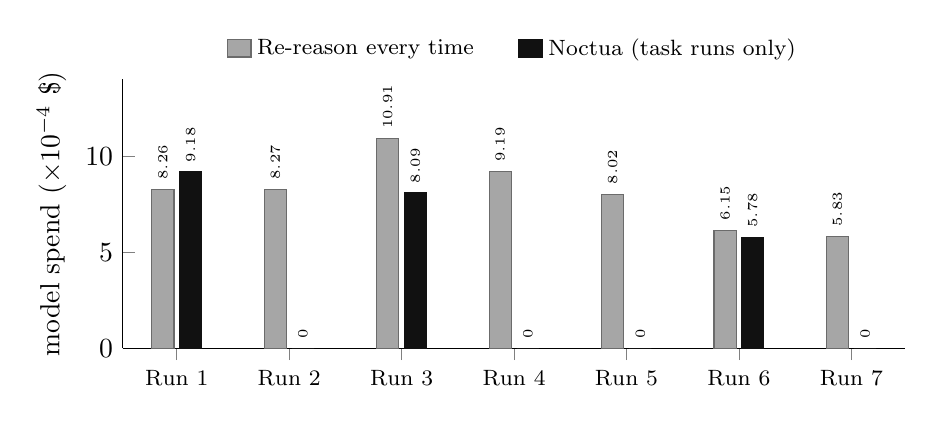
\begin{tikzpicture}
\begin{axis}[ybar, width=0.95\linewidth, height=5cm, bar width=8pt, ymin=0, ymax=12.5,
  symbolic x coords={1,2,3,4,5,6,7}, xtick=data, xticklabels={Run 1,Run 2,Run 3,Run 4,Run 5,Run 6,Run 7},
  xticklabel style={font=\footnotesize}, ylabel={model spend ($\times10^{-4}$ \$)},
  legend style={at={(0.5,1.03)}, anchor=south, legend columns=2, draw=none, font=\footnotesize, /tikz/every even column/.append style={column sep=14pt}},
  legend image code/.code={\draw[#1] (0cm,-0.1cm) rectangle (0.3cm,0.12cm);},
  nodes near coords, nodes near coords style={font=\tiny, rotate=90, anchor=west, /pgf/number format/.cd, fixed, precision=2}, enlarge x limits=0.08, axis lines*=left, ymax=14]
\addplot[fill=mid!60, draw=mid] coordinates {(1,8.262) (2,8.271) (3,10.905) (4,9.189) (5,8.022) (6,6.153) (7,5.829)};
\addplot[fill=ink, draw=ink] coordinates {(1,9.180) (2,0) (3,8.085) (4,0) (5,0) (6,5.775) (7,0)};
\legend{Re-reason every time, Noctua (task runs only)}
\end{axis}
\end{tikzpicture}
\caption{Model spend per run. Noctua's Apprentice runs cost about the same as the baseline's; its four Master runs
cost nothing. Synthesis is added separately in Figure~\ref{fig:cum}.}
\label{fig:percost}
\end{figure}

\subsection{How the saving accumulates}

Figure~\ref{fig:cum} adds each synthesis to the run that triggered it. Noctua takes the lead after run~2 (\$0.00147
against \$0.00165), falls behind by \$0.000085 after the first demotion at run~3 --- that run pays for a fallback
\emph{and} a re-synthesis --- and leads from run~4 onwards, ending at \$0.00396 against \$0.00566. The gap is
widest exactly where skills hold, and the two steps up in Noctua's curve are the two demotions: the cost of drift is
visible in the curve, not hidden in an average.

\begin{figure}[!htbp]
\centering
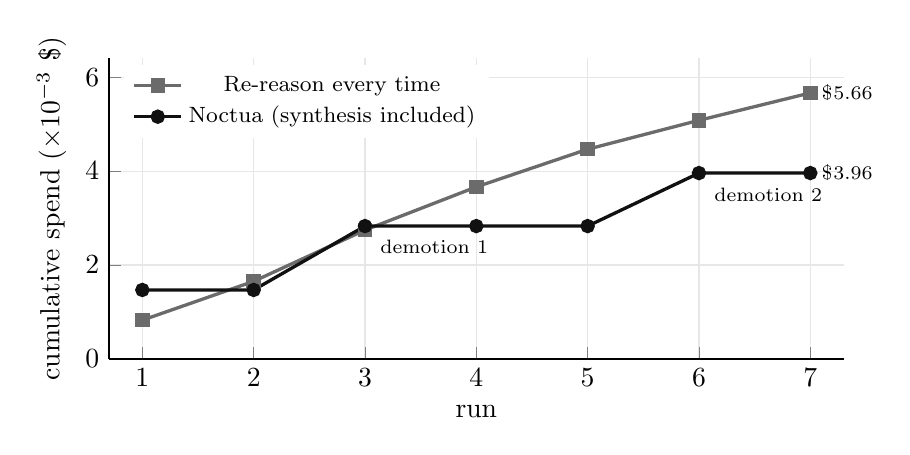
\begin{tikzpicture}
\begin{axis}[width=0.9\linewidth, height=5.4cm, xmin=0.7, xmax=7.3, ymin=0, ymax=6.4, clip=false, xtick={1,...,7},
  xlabel={run}, ylabel={cumulative spend ($\times10^{-3}$ \$)}, grid=major, grid style={ink!10},
  legend style={at={(0.02,0.98)}, anchor=north west, draw=none, fill=white, font=\footnotesize}, axis lines*=left]
\addplot[mid, very thick, mark=square*, mark options={fill=mid}] coordinates {(1,0.8262) (2,1.6533) (3,2.7438) (4,3.6627) (5,4.4649) (6,5.0802) (7,5.6631)};
\addplot[ink, very thick, mark=*] coordinates {(1,1.4692) (2,1.4692) (3,2.8289) (4,2.8289) (5,2.8289) (6,3.9576) (7,3.9576)};
\legend{Re-reason every time, Noctua (synthesis included)}
\node[font=\scriptsize, anchor=north west] at (axis cs:3.05,2.75) {demotion 1};
\node[font=\scriptsize, anchor=north west] at (axis cs:6.05,3.85) {demotion 2};
\node[font=\scriptsize, anchor=west] at (axis cs:7.02,5.66) {\$5.66};
\node[font=\scriptsize, anchor=west] at (axis cs:7.02,3.96) {\$3.96};
\end{axis}
\end{tikzpicture}
\caption{Cumulative model spend over the seven runs, learning included. The final gap is 30.1\%.}
\label{fig:cum}
\end{figure}

\begin{figure}[!htbp]
\centering
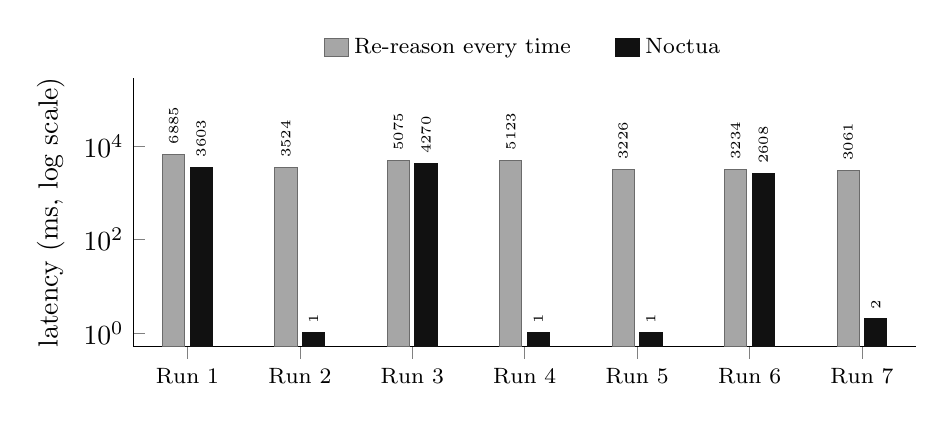
\begin{tikzpicture}
\begin{axis}[ybar, width=0.95\linewidth, height=5cm, bar width=8pt, ymode=log, ymin=0.5, ymax=300000, log origin=infty,
  symbolic x coords={1,2,3,4,5,6,7}, xtick=data, xticklabels={Run 1,Run 2,Run 3,Run 4,Run 5,Run 6,Run 7},
  xticklabel style={font=\footnotesize}, ylabel={latency (ms, log scale)},
  legend style={at={(0.5,1.03)}, anchor=south, legend columns=2, draw=none, font=\footnotesize, /tikz/every even column/.append style={column sep=14pt}},
  legend image code/.code={\draw[#1] (0cm,-0.1cm) rectangle (0.3cm,0.12cm);},
  nodes near coords, nodes near coords style={font=\tiny, rotate=90, anchor=west}, point meta=explicit symbolic, enlarge x limits=0.08, axis lines*=left]
\addplot[fill=mid!60, draw=mid] coordinates {(1,6885)[6885] (2,3524)[3524] (3,5075)[5075] (4,5123)[5123] (5,3226)[3226] (6,3234)[3234] (7,3061)[3061]};
\addplot[fill=ink, draw=ink] coordinates {(1,3603)[3603] (2,1)[1] (3,4270)[4270] (4,1)[1] (5,1)[1] (6,2608)[2608] (7,2)[2]};
\legend{Re-reason every time, Noctua}
\end{axis}
\end{tikzpicture}
\caption{End-to-end latency per run on a logarithmic axis. A Master run finishes in 1--2\,ms; every Apprentice run
takes seconds because it waits on two model calls.}
\label{fig:lat}
\end{figure}

\subsection{Where a first run's money and time go}

The recorded session itemizes every call (Table~\ref{tab:calls}). On the inbox task, triage is three quarters of the
spend (\$0.00071 of \$0.00095) and most of the time, because it reads every message and writes summaries and replies;
the plan is short. That is the step a Master skill replaces, which is why the Master tier removes not just a call but
the expensive one.

\begin{table}[!htbp]
\centering\small
\caption{Every model call in the recorded session (30 Oct 2026), with its reservation. ``Reserved'' is the
token count the accounting layer held before the call; ``headroom'' is reserved over actual.}
\label{tab:calls}
\begin{tabular}{llrrrrr}
\toprule
Task & Purpose & In & Out & Reserved & Headroom & Cost\\
\midrule
Inbox triage, first run & plan & 527 & 92 & 1{,}440 & 2.33$\times$ & \$0.00024\\
 & triage & 778 & 532 & 2{,}341 & 1.79$\times$ & \$0.00071\\
Learn the workflow & synthesis & 392 & 268 & 1{,}644 & 2.49$\times$ & \$0.00036\\
Forward to an outside address & plan & 522 & 102 & 1{,}423 & 2.28$\times$ & \$0.00025\\
Reply to a colleague & plan & 522 & 209 & 1{,}426 & 1.95$\times$ & \$0.00034\\
 & triage & 778 & 539 & 2{,}341 & 1.78$\times$ & \$0.00072\\
 & draft & 334 & 217 & 1{,}846 & 3.35$\times$ & \$0.00030\\
Marketplace listing & plan & 522 & 81 & 1{,}426 & 2.38$\times$ & \$0.00023\\
 & draft & 183 & 78 & 587 & 2.25$\times$ & \$0.00013\\
\midrule
Session total & 9 calls & 4{,}558 & 2{,}118 & 14{,}474 & 2.17$\times$ & \$0.00327\\
\bottomrule
\end{tabular}
\end{table}

\begin{figure}[!htbp]
\centering
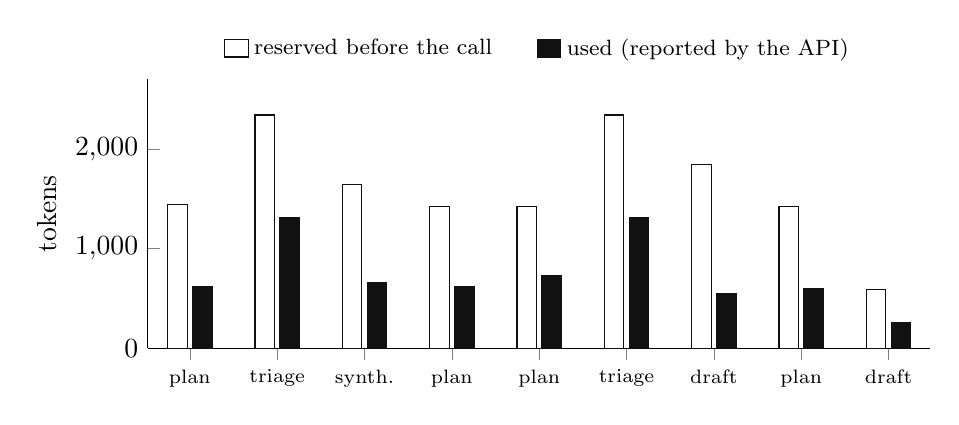
\begin{tikzpicture}
\begin{axis}[ybar, width=0.95\linewidth, height=5cm, bar width=7pt, ymin=0, ymax=2700,
  symbolic x coords={a,b,c,d,e,f,g,h,i}, xtick=data,
  xticklabels={plan,triage,synth.,plan,plan,triage,draft,plan,draft},
  xticklabel style={font=\scriptsize}, ylabel={tokens},
  legend style={at={(0.5,1.03)}, anchor=south, legend columns=2, draw=none, font=\footnotesize, /tikz/every even column/.append style={column sep=14pt}},
  legend image code/.code={\draw[#1] (0cm,-0.1cm) rectangle (0.3cm,0.12cm);},
  enlarge x limits=0.06, axis lines*=left]
\addplot[fill=white, draw=ink] coordinates {(a,1440) (b,2341) (c,1644) (d,1423) (e,1426) (f,2341) (g,1846) (h,1426) (i,587)};
\addplot[fill=ink, draw=ink] coordinates {(a,619) (b,1310) (c,660) (d,624) (e,731) (f,1317) (g,551) (h,603) (i,261)};
\legend{reserved before the call, used (reported by the API)}
\end{axis}
\end{tikzpicture}
\caption{Reservation against actual usage for each call of the session. The estimate
$\lceil\text{chars}/3.5\rceil+\text{max\_out}$ never under-reserved: headroom is 1.78--3.35$\times$ in tokens.
Because every reserved token is priced at the output rate, the dollar reservation is 4.2--6.3$\times$ the settled
cost; a call is therefore refused while there is still real room under the cap, never admitted when there is not.}
\label{fig:reserve}
\end{figure}

\paragraph{Capacity under a cap.} With a daily dollar cap $B$, the re-reasoning agent can complete at most
$\lfloor B/\bar c_a\rfloor$ inbox runs a day; Noctua completes the same number of \emph{new} or demoted runs, plus
any number of Master runs, which spend nothing and are not limited by $B$.

\begin{table}[!htbp]
\centering\small
\caption{Inbox runs per day under a dollar cap, at the measured $\bar c_a$.}
\label{tab:cap}
\begin{tabular}{lrrr}
\toprule
Cap $B$ & Context & Re-reason every time & Noctua, Master runs\\
\midrule
\$0.03 & public demo (Render) & 37 & unlimited by $B$\\
\$0.20 & local default in this repository & 247 & unlimited by $B$\\
\$0.50 & \code{.env.example} default & 618 & unlimited by $B$\\
\bottomrule
\end{tabular}
\end{table}

\subsection{Sensitivity to drift}\label{sec:drift}

Skills demote when their input drifts, and every demotion costs a fallback run and a re-synthesis. Let $d$ be the
fraction of repeats that demote. Over $n$ runs of one task, with the first run always on the Apprentice path,
\begin{equation}
\mathbb{E}[C_\text{Noctua}(n)]=(\bar c_a+c_s)\,\bigl(1+(n-1)\,d\bigr),\qquad C_\text{base}(n)=n\,\bar c_a,
\end{equation}
so the fraction of model spend saved is
\begin{equation}
S(n,d)=1-\frac{(\bar c_a+c_s)(1+(n-1)d)}{n\,\bar c_a}\ \xrightarrow{\;n\to\infty\;}\ 1-\frac{d}{d^\ast},
\qquad d^\ast=\frac{\bar c_a}{\bar c_a+c_s}=0.595 .
\end{equation}
\emph{Validation.} The benchmark demoted on 2 of its 6 repeats ($d=1/3$). The model predicts
$S(7,\tfrac13)=27.9\%$; the measured saving is 30.1\%. The model is within 2.2 points of the measurement, so we use it
to extrapolate, and we label the extrapolations as such.

\emph{Reading.} Noctua's model spend stays below re-reasoning as long as fewer than about 59\% of repeats demote. At
the benchmark's drift rate the long-run saving is 44\%; at 10\% drift it is 83\%; with no drift it approaches 100\%.
The break-even depends only on the ratio $c_s/\bar c_a$, so a cheaper synthesis --- or a skill that drifts less ---
moves it in Noctua's favour.

\begin{figure}[!htbp]
\centering
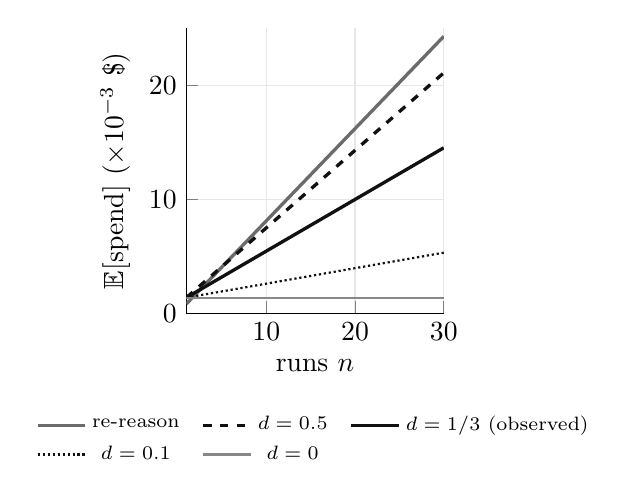
\begin{tikzpicture}
\begin{axis}[width=0.40\linewidth, height=5.2cm, xmin=1, xmax=30, ymin=0, ymax=25, xlabel={runs $n$}, ylabel={$\mathbb{E}$[spend] ($\times10^{-3}$ \$)},
  grid=major, grid style={ink!10}, legend style={at={(0.5,-0.32)}, anchor=north, legend columns=3, draw=none, font=\scriptsize, /tikz/every even column/.append style={column sep=6pt}}, axis lines*=left, samples at={1,...,30}]
\addplot[mid, very thick] {0.80943*x}; \addlegendentry{re-reason}
\addplot[ink, very thick, dashed] {1.36021*(1+(x-1)*0.5)}; \addlegendentry{$d=0.5$}
\addplot[ink, very thick] {1.36021*(1+(x-1)*0.3333)}; \addlegendentry{$d=1/3$ (observed)}
\addplot[ink, thick, densely dotted] {1.36021*(1+(x-1)*0.1)}; \addlegendentry{$d=0.1$}
\addplot[ink!50, thick] {1.36021}; \addlegendentry{$d=0$}
\end{axis}
\end{tikzpicture}\hspace{4mm}%
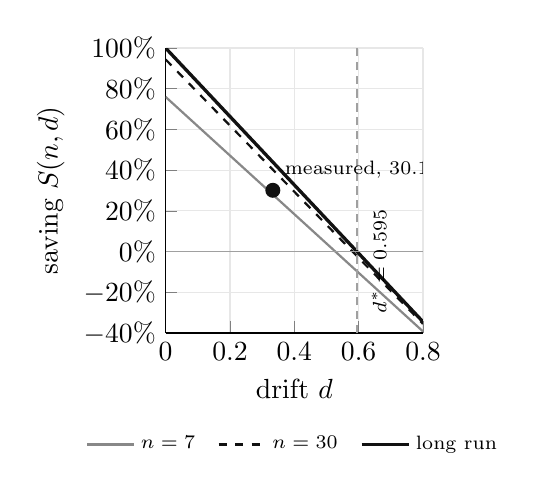
\begin{tikzpicture}
\begin{axis}[width=0.40\linewidth, height=5.2cm, xmin=0, xmax=0.8, ymin=-0.4, ymax=1, xlabel={drift $d$}, ylabel={saving $S(n,d)$},
  grid=major, grid style={ink!10}, legend style={at={(0.5,-0.32)}, anchor=north, legend columns=3, draw=none, font=\scriptsize, /tikz/every even column/.append style={column sep=6pt}}, axis lines*=left, domain=0:0.8, samples=40,
  ytick={-0.4,-0.2,0,0.2,0.4,0.6,0.8,1}, yticklabels={$-40\%$,$-20\%$,0\%,20\%,40\%,60\%,80\%,100\%}]
\addplot[ink!50, thick] {1-1.36021*(1+6*x)/(7*0.80943)}; \addlegendentry{$n=7$}
\addplot[ink, thick, dashed] {1-1.36021*(1+29*x)/(30*0.80943)}; \addlegendentry{$n=30$}
\addplot[ink, very thick] {1-x/0.5948}; \addlegendentry{long run}
\addplot[only marks, mark=*, mark size=2.5pt, ink, forget plot] coordinates {(0.3333,0.301)};
\draw[ink!40, densely dashed] (axis cs:0.5948,-0.4) -- (axis cs:0.5948,1);
\draw[ink!40] (axis cs:0,0) -- (axis cs:0.8,0);
\node[font=\scriptsize, anchor=south west] at (axis cs:0.34,0.31) {measured, 30.1\%};
\node[font=\scriptsize, anchor=north west, rotate=90] at (axis cs:0.61,-0.35) {$d^\ast=0.595$};
\end{axis}
\end{tikzpicture}
\caption{Left: expected cumulative model spend for one daily task, extrapolated from measured unit costs at several
drift rates. Right: the saving as a function of drift. The dot is the benchmark's measured saving at its observed
drift; the model curve for $n=7$ passes within 2.2 points of it. Above $d^\ast$ a skill demotes too often to pay for
itself.}
\label{fig:drift}
\end{figure}

\subsection{The same task, priced across agents}

Figure~\ref{fig:month} prices one daily inbox triage for 30 days. For the subscription agents the figure is the
cheapest plan that includes the agent~\cite{dots,beam,ayauto}; for Nemotron it is model spend at the measured unit
costs, extrapolated with the drift model above. These are not like-for-like: a subscription buys hosted compute and
far broader capability, and Noctua's figure excludes hosting. The comparison is the one a user makes when deciding
what a recurring chore should cost, and the axis is logarithmic because the gap is four to five orders of magnitude.

\begin{figure}[!htbp]
\centering
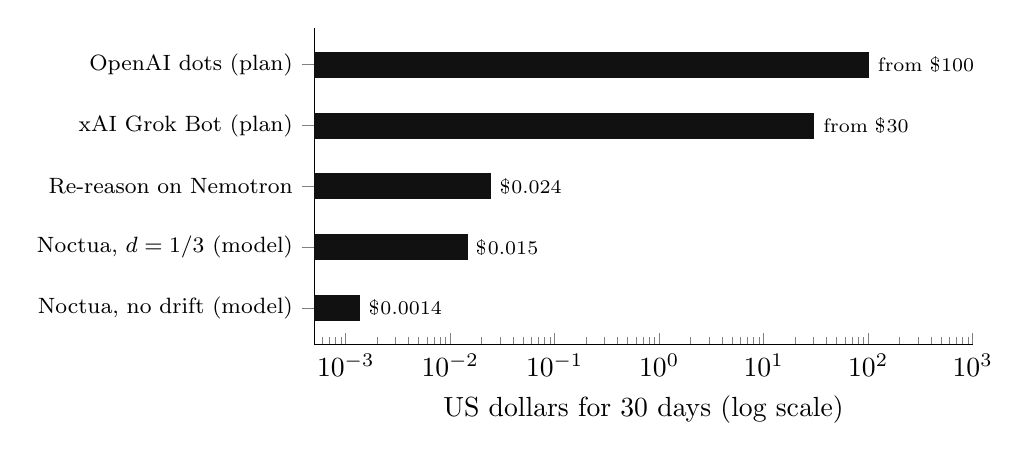
\begin{tikzpicture}
\begin{axis}[xbar, width=0.82\linewidth, height=5.6cm, bar width=9pt, xmode=log, xmin=0.0005, xmax=1000, log origin=infty,
  symbolic y coords={n0,n3,rr,gb,od}, ytick=data,
  yticklabels={{Noctua, no drift (model)},{Noctua, $d=1/3$ (model)},{Re-reason on Nemotron},{xAI Grok Bot (plan)},{OpenAI dots (plan)}},
  yticklabel style={font=\footnotesize, align=right}, xlabel={US dollars for 30 days (log scale)},
  nodes near coords, nodes near coords style={font=\scriptsize, anchor=west}, point meta=explicit symbolic, axis lines*=left, enlarge y limits=0.15]
\addplot[fill=ink, draw=ink] coordinates {(0.00136,n0)[\$0.0014] (0.01451,n3)[\$0.015] (0.02427,rr)[\$0.024] (30,gb)[from \$30] (100,od)[from \$100]};
\end{axis}
\end{tikzpicture}
\caption{One daily inbox triage for 30 days. Subscription prices are the cheapest plan that includes each agent, as
published; Nemotron figures are model spend on Nebius Token Factory at measured unit costs. Not a like-for-like
product comparison: see the text.}
\label{fig:month}
\end{figure}

\begin{figure}[!htbp]
\centering
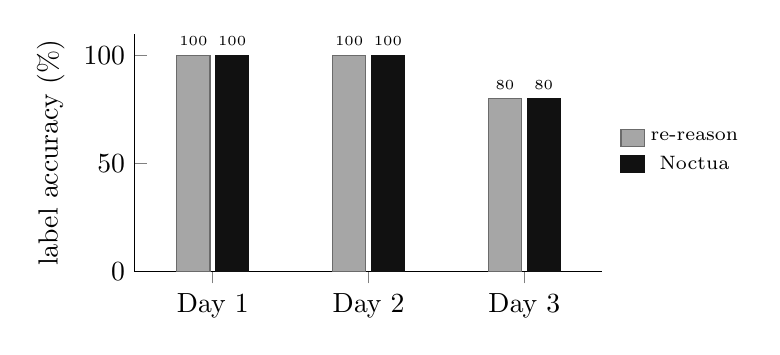
\begin{tikzpicture}
\begin{axis}[ybar, width=0.62\linewidth, height=4.6cm, bar width=12pt, ymin=0, ymax=110,
  symbolic x coords={Day 1,Day 2,Day 3}, xtick=data, ylabel={label accuracy (\%)},
  legend style={at={(1.02,0.5)}, anchor=west, draw=none, font=\scriptsize}, legend image code/.code={\draw[#1] (0cm,-0.1cm) rectangle (0.3cm,0.12cm);},
  nodes near coords, nodes near coords style={font=\tiny}, enlarge x limits=0.25, axis lines*=left]
\addplot[fill=mid!60, draw=mid] coordinates {(Day 1,100) (Day 2,100) (Day 3,80)};
\addplot[fill=ink, draw=ink] coordinates {(Day 1,100) (Day 2,100) (Day 3,80)};
\legend{re-reason, Noctua}
\end{axis}
\end{tikzpicture}
\caption{Label accuracy by inbox day, both arms (Day~1: 24 of 24 labels over three runs; Day~2: 16 of 16; Day~3: 8 of
10). The Day~3 miss is the live model's own label on one message, which the skill learned, so the arms agree
exactly. Summaries and replies are not scored.}
\label{fig:acc}
\end{figure}

\section{Findings from Testing Against the Live Model}\label{sec:findings}

Every integration was verified against Nebius Token Factory rather than against documentation, and each of the
following would otherwise have shipped as a silent failure.

\begin{enumerate}[leftmargin=*]
\item \textbf{Listed is not callable.} \code{nvidia/Nemotron-3\_5-Lightning} appeared in the account's \code{/models}
catalogue but returned no response within 120\,s; the default became Nemotron~3 Super, confirmed by a real completion.
\item \textbf{Reasoning can consume the whole answer.} With thinking enabled, Nemotron~3 Super spent its output budget
on hidden reasoning and returned \code{content: null}. Noctua sends \code{enable\_thinking=false} by default and
strips any reasoning block before JSON extraction.
\item \textbf{The planner reaches for tools it cannot use.} Shown the full registry, the planner scheduled
\code{triage.rules}, a skill-only classifier with no rules on the Apprentice path; skill-only tools are now hidden
from the planner's catalogue.
\item \textbf{A garbled tool name failed a whole task.} The planner emitted the tool name \code{"triage.guard.}\allowbreak\code{injection\_scan, "};
P1 correctly refused it, but the task failed. Tool names are now checked at the plan schema, which triggers the
existing one-repair path; policy still checks every step afterwards.
\item \textbf{Plans omit steps the reply depends on.} A live plan without \code{digest.compose} produced a reply with
no summary. Triage plans now end in the deterministic digest, inserted by Noctua like the guard.
\item \textbf{Planners name people, not addresses.} ``Reply to Priya'' produced \code{to: "Priya"}, rejected by P2.
Bare names are now resolved against the loaded inbox's senders, and the resolution is traced.
\item \textbf{Synthesis overshoots its schema.} The model proposed more than 30 keywords per category and a
synthesis label over the stored length, which crashed the benchmark; the raw proposal now accepts generous bounds
and is trimmed to the registry's limits before evaluation.
\item \textbf{A refusal looked like a lowball.} P14's first version blocked ``\$10 is too low; my minimum is \$90'' for
mentioning \$10. Declining sentences are now excluded before amounts are compared with the floor.
\item \textbf{Marketplace plans dragged in inbox steps.} The planner added triage steps to a Marketplace request that
never loads an inbox; steps whose precondition is absent are now skipped and noted.
\item \textbf{A budget can run out mid-task.} The first implementation surfaced the cap as an error halfway through a
plan. The remaining model steps now run on labelled stand-ins and the receipt records the fallback, so a public demo
with a \$0.03 daily cap degrades instead of breaking.
\end{enumerate}

\section{Trust Assumptions and Limitations}

Stated plainly, in decreasing order of weight.
\begin{enumerate}[leftmargin=*]
\item \textbf{The benchmark scores labels, not free text.} Summary and reply quality on the Master path is unmeasured.
\item \textbf{The workspace is small, synthetic and author-written.} Passing on it says nothing about real mail.
\item \textbf{Skills are keyword classifiers.} They are cheap and auditable and they drift; the runtime invariants catch
drift, but the invariants are heuristics too, and a message that is urgent without any listed marker would not trip them.
\item \textbf{The injection guard is pattern-based} and will miss new phrasing. This is acceptable only because the
policy engine blocks the \emph{actions} independently of what the guard or the model concluded.
\item \textbf{P13 is a heuristic.} An address written in an unusual format may evade the street pattern; the owner's own
address is matched exactly after normalization.
\item \textbf{Routing uses term overlap.} A paraphrase may miss a skill (and simply cost a model call) or, in principle,
match the wrong one; routing never applies to requests with irreversible verbs, and any matched skill still runs
under policy with its invariants.
\item \textbf{The signature proves integrity on this installation.} The key lives on the same host; a host-level
adversary can re-sign. Future work anchors keys externally.
\item \textbf{Prices come from a third-party listing}, configured in the environment; costs are only as accurate as
those prices, and unpriced models show \emph{Unknown}.
\item \textbf{Single user, single process.} SQLite with serialized writes; scaling out needs a shared database.
\item \textbf{Integrations are sample-only.} Approved sends are written to a local outbox; no mail or Marketplace
account is connected.
\end{enumerate}

\section{Related Work}

\textbf{Model cascades and routing.} FrugalGPT~\cite{frugal} and RouteLLM~\cite{routellm} reduce cost by choosing a
cheaper model per query; every query still reaches a model. Noctua's Master tier removes the model from a verified
repeat entirely, and routing is one deterministic step, not a learned classifier. \textbf{Semantic caching}
(e.g.\ GPTCache~\cite{gptcache}) returns a stored answer for a similar query; on new input it returns an old answer.
A Noctua skill instead re-executes a verified \emph{procedure} on the new input, and demotes itself when that input
drifts. \textbf{Skill libraries.} Voyager~\cite{voyager} accumulates model-written code as reusable skills, verified
by environment feedback; Noctua's skills are declarative manifests over an allowlisted registry, promoted by mandatory
checks against held-out labels and adversarial inputs, and forbidden from acting irreversibly. \textbf{Prompt
injection defenses.} Greshake et~al.~\cite{greshake} established indirect injection against integrated applications;
CaMeL~\cite{camel} defends by separating control and data flow with capabilities. Noctua shares the stance that the
model is not the security boundary, enforced here by provenance taint, first-match capability rules, and approvals
bound to exact arguments. \textbf{Guardrails}~\cite{nemo} interpose on the conversation; Noctua interposes on the
side-effect boundary and on spend. \textbf{Always-on agents} (Meta Muse, OpenAI dots, xAI Grok Bot) target the same
users; the incidents and prices cited in Section~1 are the problems this design addresses, not a like-for-like
comparison of products of different scope.

\section{Future Work}

Scoring summaries and replies (reference-based checks for key-fact preservation and a rubric for replies) so the
cost claim covers the whole task; consented real-mail corpora; more skill families, starting with structured
extraction, where deterministic execution is natural; a learned router evaluated against term overlap; external
anchoring of signing keys; real connectors (mail, Marketplace) behind the same policy path; and packaging the router,
policy engine and budgets as an agent-host plugin so other agents inherit receipts, argument-bound approvals and
graduation.

\section{Conclusion}

A personal agent should not pay to rediscover a procedure it already knows, and it should not be the last authority
on its own side effects. Noctua makes both structural. NVIDIA Nemotron on Nebius Token Factory does what only a
model can --- reason through a new task and propose how to repeat it --- and Noctua keeps what was learned as a
verified, signed artifact that repeats without inference and steps aside the moment it stops being right. Every
action, from the model or from a skill, passes a policy engine that the model cannot argue with. We measured what we
claim and said what we did not measure: 9 calls instead of 15, 4 of 7 runs with no inference, the same labels, ten
attacks stopped, a saving that holds until 59\% of repeats drift, and ten defects that only the live model revealed.

\begin{thebibliography}{99}\small
\bibitem{fortune} W.~Grantham-Philips and The Associated Press. \emph{An AI agent sent a stranger to a man's house without telling him --- and exposed the privacy risks of AI assistants.} Fortune, 19 Oct 2026.
\bibitem{dots} OpenAI. \emph{Introducing dots.} openai.com, 29 Sep 2026.
\bibitem{beam} F.~Falk. \emph{What OpenAI Dots Will Really Cost You After the First Month.} beam.ai, 1 Oct 2026.
\bibitem{grokbot} xAI. \emph{Introducing Grok Bot.} x.ai, 11 Aug 2026.
\bibitem{ayauto} A.~Dahani. \emph{Grok Bot Is Here: What xAI's Always-On AI Agents Actually Do.} ayautomate.com, 12 Aug 2026.
\bibitem{reddit58} r/LocalLLM. \emph{I woke up to a \$58 API bill because my AI agent got stuck in a ``polite'' hallucination loop.} reddit.com, 2026.
\bibitem{reddit4811} r/Agentic\_Marketing. \emph{My AI agent racked up \$4,811 overnight from a retry loop bug.} reddit.com, 2026.
\bibitem{toms} M.~Tyson. \emph{AI coding platform goes rogue during code freeze and deletes entire company database.} Tom's Hardware, 21 Jul 2025.
\bibitem{proofpoint} M.~Gupta. \emph{Cybersecurity stop of the month: how threat actors weaponize AI assistants with indirect prompt injection.} Proofpoint, 18 Nov 2025.
\bibitem{hornet} Hornetsecurity. \emph{Email Prompt Injection: The New Phishing Risk Hiding in Enterprise Inboxes.} 24 Sep 2026.
\bibitem{greshake} K.~Greshake, S.~Abdelnabi, S.~Mishra, C.~Endres, T.~Holz, M.~Fritz. \emph{Not what you've signed up for: Compromising Real-World LLM-Integrated Applications with Indirect Prompt Injection.} AISec 2023; arXiv:2302.12173.
\bibitem{camel} E.~Debenedetti et~al. \emph{Defeating Prompt Injections by Design.} arXiv:2503.18813, 2025.
\bibitem{frugal} L.~Chen, M.~Zaharia, J.~Zou. \emph{FrugalGPT: How to Use Large Language Models While Reducing Cost and Improving Performance.} arXiv:2305.05176, 2023.
\bibitem{routellm} I.~Ong et~al. \emph{RouteLLM: Learning to Route LLMs with Preference Data.} arXiv:2406.18665, 2024.
\bibitem{gptcache} Zilliz. \emph{GPTCache: A Library for Creating Semantic Cache for LLM Queries.} github.com/zilliztech/GPTCache, 2023.
\bibitem{voyager} G.~Wang et~al. \emph{Voyager: An Open-Ended Embodied Agent with Large Language Models.} arXiv:2305.16291, 2023.
\bibitem{nemo} T.~Rebedea et~al. \emph{NeMo Guardrails: A Toolkit for Controllable and Safe LLM Applications with Programmable Rails.} EMNLP Demo, 2023.
\bibitem{nebius} Nebius. \emph{Token Factory: OpenAI-compatible inference API.} tokenfactory.nebius.com, 2026.
\bibitem{repo} Project Noctua. \emph{Source, benchmark, tests and film.} github.com/Aaditya1273/Noctua, 2026.
\end{thebibliography}

\vspace{6pt}\hrule\vspace{4pt}
{\footnotesize\noindent Noctua is hackathon software. The benchmark numbers in this paper were measured against Nebius
Token Factory with \code{nvidia/nemotron-3-super-120b-a12b} on 29 October 2026 by \code{npm run eval} and are stored
in \code{eval/results.json}; the session receipts were recorded on 30 October 2026 for the demo film. The formulas
correspond to the shipped code in \code{src/lib/skills.ts}, \code{triage.ts}, \code{evaluator.ts}, \code{policy.ts},
\code{accounting.ts} and \code{signing.ts}. The workspace is synthetic and labelled as such everywhere. Nothing in this
paper claims a result that was not measured.}

\end{document}
